\documentclass{../../missal-sheet}

\begin{document}

\chapter*{Evangelium Passionis et Mortis domini Secundum Matth\'{\ae}um}

\begin{center}
 Matthew 26, 36-75; 27, 1-60
\end{center}

\begin{rubricbox}
{\color{red} The Gospel procession having taken place, the clerics assemble themselves on the Gospel side, facing liturgical north. The Passion Narrative is chanted, with \textit{four} parts contributing: The Chronicler (symbolized by a letter `C'), Christ (symbolized by a `\maltese'), a singular Synagogue part (symbolized by a `S'), and a plural Synagogue part, known as the `Turba', literally meaning `crowd' (symbolized by a `T').  The Chronicler begins the chanting of the Passion Narrative. For ease of chanting, the singular Synagogue part has been tranposed down a perfect fourth from its original setting.}
\end{rubricbox}

% Page 1:

\gresetinitiallines{1}
\gregorioscore{matthew_passion_1}

% Page 2:

\gresetinitiallines{0}
\gregorioscore{matthew_passion_2}

% Page 3:

\gresetinitiallines{0}
\gregorioscore{matthew_passion_3}

% Page 4:

\gresetinitiallines{0}
\gregorioscore{Victoria/matthew_passion_4a}

{\color{red}\textit{The Turba sings the following:}}

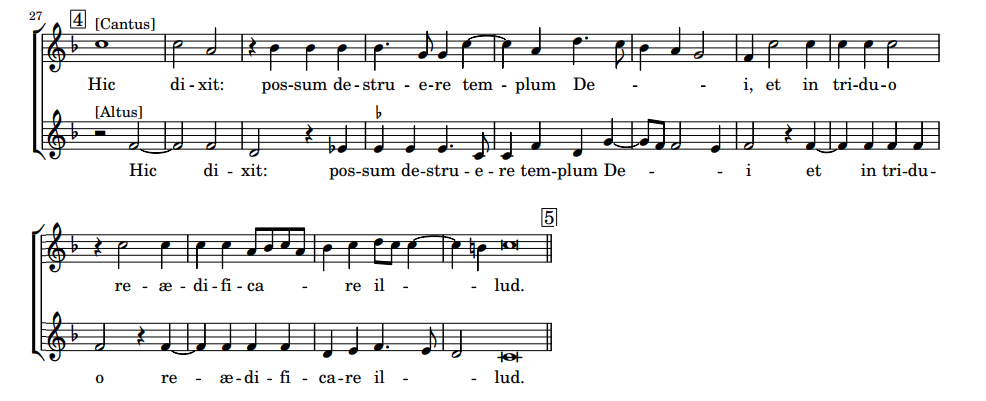
\includegraphics[width=\textwidth]{Victoria/Polyphony/turba1_fixed}

\gresetinitiallines{0}
\gregorioscore{Victoria/matthew_passion_4b}

% Page 5:

\gresetinitiallines{0}
\gregorioscore{Victoria/matthew_passion_5a}

{\color{red}\textit{Turba:}}

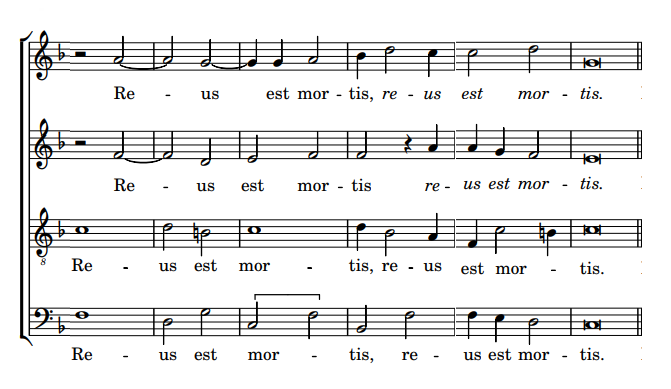
\includegraphics[width=\textwidth]{Victoria/Polyphony/turba2_fixed}

\gresetinitiallines{0}
\gregorioscore{Victoria/matthew_passion_5b}

\vfill\pagebreak

% Page 6:

{\color{red}\textit{Turba:}}

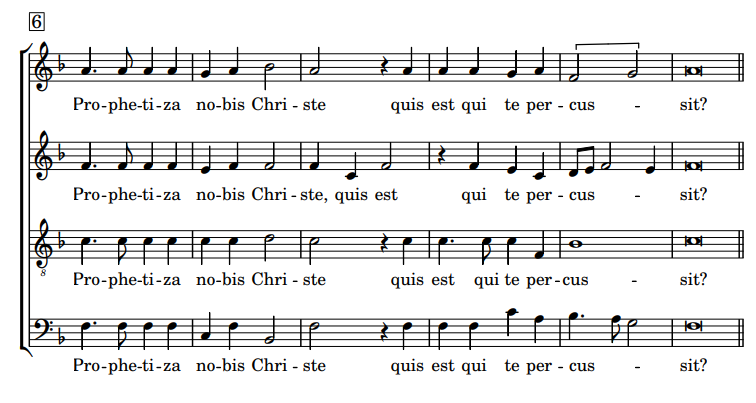
\includegraphics[width=\textwidth]{Victoria/Polyphony/turba3_fixed}

\gresetinitiallines{0}
\gregorioscore{Victoria/matthew_passion_6a}

{\color{red}\textit{Turba:}}

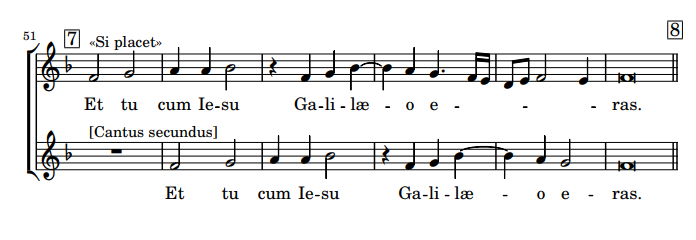
\includegraphics[width=\textwidth]{Victoria/Polyphony/turba4_fixed}

\gresetinitiallines{0}
\gregorioscore{Victoria/matthew_passion_6b}

\vfill\pagebreak

% Page 7:

{\color{red}\textit{Turba:}}

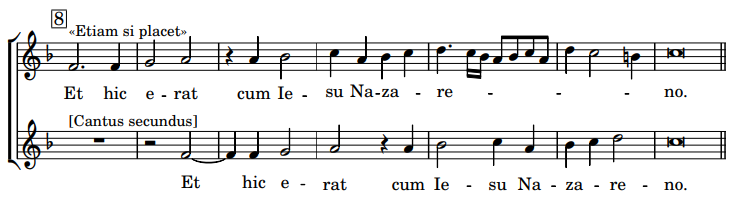
\includegraphics[width=\textwidth]{Victoria/Polyphony/turba5_fixed}

\end{document}